
\documentclass[11pt]{memoir} % use larger type; default would be 10pt


%inkluderte pakker
\usepackage[utf8]{inputenc}
\usepackage{hyperref}
\usepackage{paralist}
\usepackage{graphicx}
\usepackage[margin=8pt,font=small,labelfont=bf]{caption}

%slutt på pakkene

\title{- Prosjektoppgave - \\ Samfunnsmedisinkurs C \\ Oslo, 11.- 13. November 2013}
\author{Pål Ager-Wick \\ Kommuneoverlege Øvre- og Nedre Eiker}
\date{} % Activate to display a given date or no date (if empty),
         % otherwise the current date is printed 

\begin{document}
%%Her begynner oversettelsen til norsk
			\renewcommand{\chaptername}{Del}
            \renewcommand{\contentsname}{Innhold}
            \renewcommand\listfigurename{Illustrasjoner}
            \renewcommand\tablename{Tabell}
			\renewcommand\listtablename{Tabeller}
            \renewcommand{\figurename}{Illustrasjon}

%%Her slutter den
\frontmatter

\maketitle

\chapter{Forord til oppgaven}
	Jeg skriver her et kort forord fordi jeg har langt overskredet sidetallet som var satt til to sider. Det er i størst grad fordi jeg velger å skrive dokumenter i et spesielt format som gjør dem mer leservennlige og lettere å disponere når man skal skrive. Jeg tror derfor at oppgaven, selv om den er på betydelig mer enn to sider, likvel vil tilsvare omlag 2 tettskrevne A4 sider.\\

	Denne programvaren er åpen. Dette standarden for innleveringer av oppgaver ved for eksempel Universitet i Oslo. Dersom det er mer interesse kan man gjøre et google søk etter LaTex, som er et programmeringsspråk som kompileres til portable datafiler(pdf).\\

	Det finnes en fullstendig versjonsoversikt som er åpent tilgjengelig på \href{http://pcjawick.github.io/Folkehelseoppgave}{GitHub}. Her kan du laste ned hele prosjektet og finne lenke til versjonsoversikten.\\

	Til slutt tillater jeg meg en tilbakemelding om at denne oppgaveteksten, som i seg selv var på 1/2 A4 side, vanskelig kan komme under 2 A4 sider på en meningsfull måte.



\newpage

\tableofcontents

\mainmatter

\chapter{Utfordringer for Nedre Eiker kommune}
	\section{Folkehelseprofilen}
		\paragraph{}
			Jeg kom inn i kommunelegejobben med erfaring fra allmennmedisin og legevaktvaktsmedisin. Folkehelse var et vagt begrep for meg og jeg hadde ingen følelse med hvordan kommunen jobbet med dette. Selve begrepet gav meg en følelse av politisk "glasur". 
%Her begynner grafikken

                    \begin{figure}[h]
                      \centering
                      	\frame{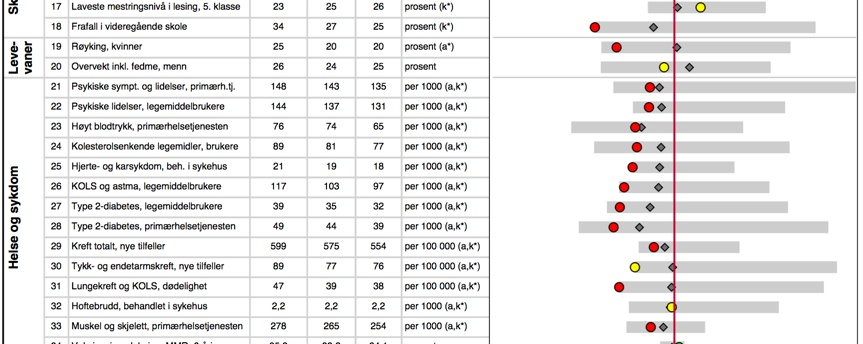
\includegraphics[width=4.7in]{./fhprofilnek.jpg}}%utklipp fra fh profilen 2013
                      \captionsetup{singlelinecheck=off}
                      \caption{Utdrag fra folkehelseprofilen i Nedre Eiker}
                      {Figuren viser et utdrag fra folkehelseprofilen i Nedre Eiker. Her er det mye å ta fatt i, men det skyldes det selektive utsnittet. Jeg ønsker å vise at folkehelseprofilen kan være vanskelig å bruke som datagrunnlag med et så mangfoldig problemområde. Omvendt kan de positive trendene være falsk positive av på grunn av metodene eller befolkningssammensetningen.\cite{fhprofil}}\label{fhprofilnekbilde}%\textit{tjenestetilbudene}.]
                    \end{figure}    

%Her slutter grafikken            
		\paragraph{}	
			Jeg mener at folkehelseprofilene er et godt utgangspunkt for å identifisere kommunale problemområder. Se illustrasjon \ref{fhprofilnekbilde} for et utsnitt av problemområdet til Nedre Eiker.
		
	\section{Eksisterende planverk}
		\paragraph{}
			Det er viktig å danne seg et bilde av eksisterende planverk.
	\section{Hvordan virkeligheten ser ut}

\chapter{Fokusområde: Fysisk helse}
	\section{Hvorfor fysisk helse?}
	\section{Hvordan måle effekten}
	\section{Suksessfaktorer}


\chapter{Gjennomføring}
	\section{Finansiering}
	\section{Administrative forutsetninger}
	\section{Første skritt på veien}

 \renewcommand{\bibname}{Kilder:}
              \begin{thebibliography}{99}

                \bibitem{Stmld47}
                  Helse- og Omsorgsdepartementet,
                  \emph{Stortingsmelding 47, 06/2009, Samhandlindlingsreformen}.
                  Hansen, Bjarne Haakon m. fl. (Minister)

                 \bibitem{fhprofil}
                  Folkehelseprofilen i Nedre Eiker
                  \emph{Folkehelseinstiuttet}.
                  

\end{thebibliography}


\end{document}